\section{Results} In the following sections we will discuss some key results;
for a more complete look at the output of the scripts, we ask that you please
consult the Appendices.

\subsection{Teleportation} The main result of the teleportation protocol is
summarized in Fig. \ref{fig:teleport_histogram}. The ideal simulation fidelities
are all within statistical error of unity, an important check to ensure that the
state, reconstructed through tomography, and post-measurement selection scheme
both are working as expected. The Noisy Simulator is modelled using the
single-qubit errors, CNOT errors and a model of readout error in each backend.
As we will continue to see with the other circuits, the noise model overestimate
the performance of the backend, but interestingly in this case, for the
Melbourne device, we find that the noise model almost matches that of the
device.

The noise model captures the error in the Burlington device much less
accurately. We would expect that Burlington would perform almost as well as
Yorktown from the estimates on the noisy simulator, but in fact it performs the
worst of the three. We suspect, as will be described in more detail below, that
this is a consequence of the number of gates needed to implement the circuit on
the real device. 

\begin{figure}[h] \centering
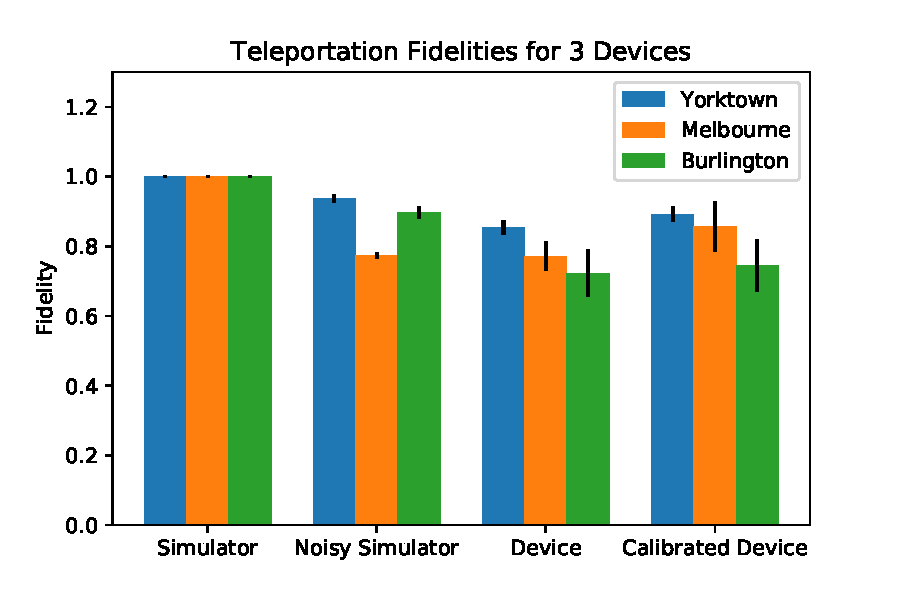
\includegraphics[width=0.48\textwidth]{images/results/teleport_histogram.pdf}
  \caption{Fidelity results for the Teleportation protocol. Error bars are
estimated by taking the variance over 15 runs of 8,192 shots each (a total of
122,880 shots). All simulation fidelities are within statistical error of
unity.}
  \label{fig:teleport_histogram}
\end{figure}

In order to check the readout calibration, it is useful to compare Pauli sets of
the different outcomes. 

\subsection{Entanglement Swapping}
\subsection{Entanglement Purification}
\subsection{Grover's Algorithm}

\begin{figure*} \centering
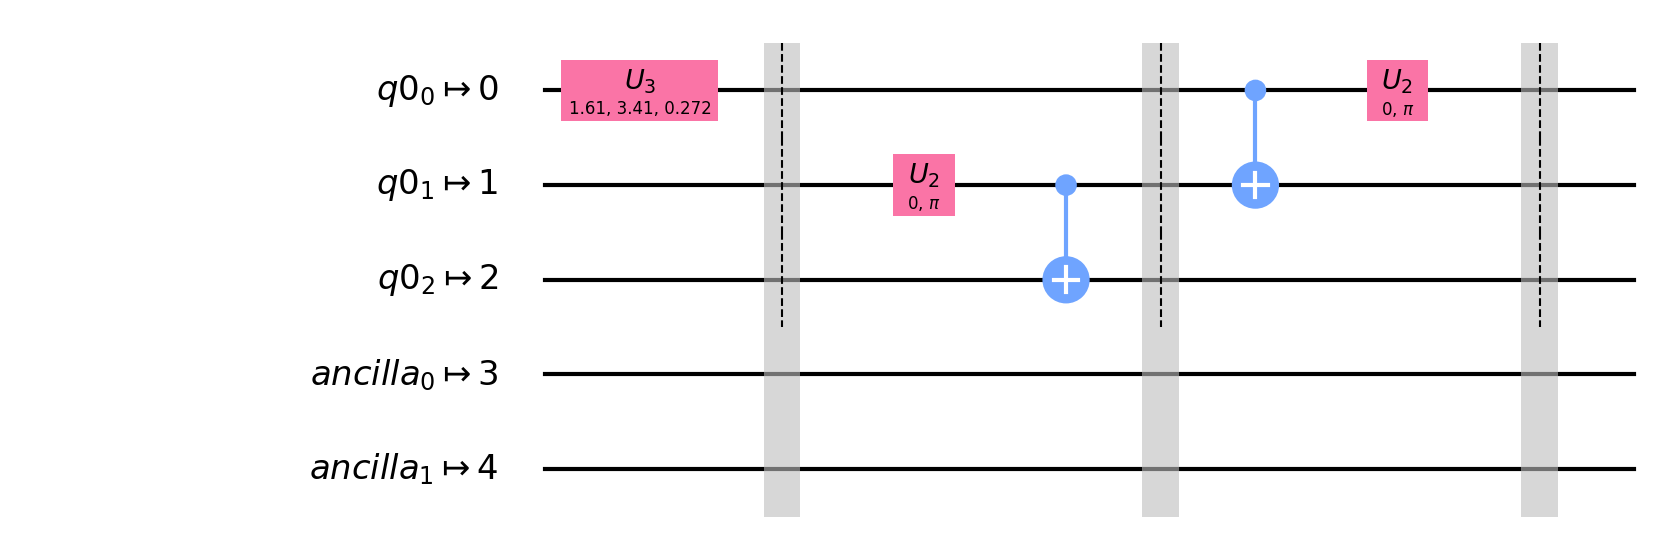
\includegraphics[width=\textwidth]{images/teleport_ibmqx2.png}
  \caption{The most densely connected 5-qubit device at IBM Q. As we will see,
equally as important as the single-qubit and CNOT error rates is the degree of
connectivity in a device. Figure from \cite{ibmq_yorktown}.}
  \label{fig:yorktown_connections}
\end{figure*}

%%% Local Variables:
%%% mode: latex
%%% TeX-master: "report"
%%% End: